\documentclass[a4paper, 10pt, conference]{ieeeconf}

\overrideIEEEmargins   % Needed to meet printer requirements.
% See the \addtolength command later in the file to balance the column lengths
% on the last page of the document

\usepackage{graphicx}  % for pdf, bitmapped graphics files
%\usepackage{epsfig}   % for postscript graphics files
%\usepackage{mathptmx} % assumes new font selection scheme installed
%\usepackage{times}    % assumes new font selection scheme installed
%\usepackage{amsmath}  % assumes amsmath package installed
%\usepackage{amssymb}  % assumes amsmath package installed




\title{ %\LARGE \bf
  Distributed Intelligent Systems: Course Project\\
  Swarm compactness maintenance using only local communication
}

\author{
  Morgan Bruhin (\texttt{morga.bruhin@epfl.com}) \\
  Merlin Nimier David (\texttt{merlin.nimier-david@epfl.com}) \\
  Krishna Raj Sapkota (\texttt{krishna.sapkota@epfl.com})
}

\begin{document}


\maketitle
\thispagestyle{empty}
\pagestyle{empty}

%%%%%%%%%%%%%%%%%%%%%%%%%%%%%%%%%%%%%%%%%%%%%%%%%%%%%%%%%%%%%%%%%%%%%%%%%%%%%%%%
\begin{abstract}
  Short, but concise description of your project and results.
\end{abstract}

\section{Introduction}
  Modelling of swarm algorithms is important since it allows us to predict the overall behaviour of the swarm as well as study the influence of individual robot parameters on the swarm behaviour. Also swarm modelling is crucial for tasks such as validation of swarm algorithms before they can be deployed in real world situation. In this project we seek to model a wirelessly connected swarm at a macroscopic level and compare it to the same algorithm implemented in sub-microscopic simulation. As a first part of the project we implemented alpha algorithm (discussed below) in webots (sub-microscopic level), as a second part we modeled the same algorithm at a macroscopic level and as a third part we implemented an additional algorithm, beta algorithm, along with behaviours such as taxis towards a beacon and beacon encapsulation.\\

  We implemented the alpha algorithm as presented in \cite{Winfield08} which is a simpler version of beta algorithm presented in \cite{Nembrini02}. In alpha algorithm robots are in a default state of forward motion until the number of connections drops below a certain threshold. All the robots are equipped with a short range radio communication device (communication range is often much smaller than the size of the swarm) and are able to ``sense'' the number of robots that are within their communication range. At every time step each robot keeps track of number of its neighbors. If the number of neighbors fall below a certain threshold (dictated by alpha parameter) the robot switches form FORWARD state to COHERENCE state. In both states obstacle avoidance is ensured with the help of IR sensors onboard the robot. FORWARD and COHERENCE states are preemptive over AVOIDANCE in that state change to FORWARD or COHERENCE while at AVOIDANCE causes the robot to immediately stop AVOIDANCE and switch to the new state.  Hence the robots behave as if they were attached to each other via an elastic band. In COHERENCE state the robot tries to recover the swarm by turning 180 degrees in place and hence moving backwards. The robot makes a random turn if the number of connections rises following a COHERENCE move to recover the swarm. One drawback of alpha algorithm is that the swarm is very sensitive to communication loss and hence tends to collapse on itself while trying to recover too often.

  Just like in alpha algorithm in beta algorithm robots are equipped with basic collision avoidance sensors and short range omnidirectional radio for communication. In addition, each robot is equipped with a beacon sensor. In terms of locomotive capabilities each robot is capable of moving forward in a straight line as well as making a turn in place with reasonable accuracy. In our simulations we use all 8 infrared sensors onboard the robot and a simple weight based Breitenberg controller to achieve obstacle avoidance behaviour. A beacon is introduced with line of sight occlusion in order to study the collective movement of swarm towards a certain point.\\

  While each robot can tell if a certain robot is in its communication range (based on exchanged messages) any kind of absolute or relative pose of neighbors is not available to the robots. Each robot broadcasts its neighborhood information (IDs of its current/latest neighbors) at a regular time interval unlike alpha algorithm where each robot only sends ``I am here'' messages. This additional information allows for a different locomotive strategy resulting in a more flexible swarm and results in many more additional emergent behaviours. In alpha algorithm we saw that as the number of robots in the swarm increases the swarm as a whole becomes more and more reactive (since robots reacts to every communication loss) and clumps together. In beta algorithm such overreactivity is overcome by exploiting the additional neighborhood information available to each robot. Unlike alpha algorithm in beta algorithm a robot reacts to a communication loss only when the lost robot is shared by less than a certain number (given by parameter ``beta'' and hence the name of the algorithm) of neighbors. In other words, as long as a good number of neighbors are in the range of the lost robot swarm recovery behaviour is not triggered. This allows the swarm to be more flexible and thus eliminates the problem of entire swarm collapsing on itself like we saw with the alpha algorithm. Additionally robots take a random heading if the number of connections rises over time.\\

  Besides submicroscopic and macroscopic modeling of alpha algorithm we also implemented beta algorithm at the submicroscopic level. We also studied movement of swarm of robots towards a beacon while ensuring obstacle avoidance. The later being an emergent property of the beta algorithm resulting from differentiation of certain robots from the rest. In section III we compare beta algorithm with alpha algorithm based on various metrics and present some visual results.

%%%%%%%%%%%%%%%%%%%%%%%%%%%%%%%%%%%%%%%%%%%%%%%%%%%%%%%%%%%%%%%%%%%%%%%%%%%%%%%%

\section{Experiments}
  \subsection{State machine}
  Present the controller's states. Explain the transitions. Explain the obstacle avoidance behavior (Braitenberg's controller).

  \subsection{Experimental setup} \label{simulations}
  We used the realistic simulation software Webots (developped by Cyberbotics, an EPFL spin-off startup). Webots offers realistic 3D rendering of scenes as well as physics simulation. We use an open (``infinite'') arena with 40 agents. Each agent is a submicroscopic-level representation of the E-Puck robot: the model is complete with each sensor, actuators, etc. We leverage realistic communication simulation to limit the range of communication to a fixed radius around each agent. Messages are delivered after a delay. However, make the symplifying assumption that messages are received as they were sent, i.e. without corruption or noise over the contents of the message.\\

  Just like in alpha algorithm in beta algorithm robots are equipped with basic collision avoidance sensors and short range omnidirectional radio for communication. In addition, each robot is equipped with a beacon sensor. In terms of locomotive capabilities each robot is capable of moving forward in a straight line as well as making a turn in place with reasonable accuracy. In our simulations we use all 8 infrared sensors on-board the robot and a simple weight based Breitenberg controller to achieve obstacle avoidance behavior. A beacon is introduced with line of sight occlusion in order to study the collective movement of swarm towards a certain point. \\
  While each robot can tell if a certain robot is in its communication range (based on exchanged messages) any kind of absolute or relative pose of neighbors is not available to the robots. Each robot broadcasts its neighborhood information (IDs of its current/latest neighbors) at a regular time interval unlike alpha algorithm where each robot only sends ``I am here!'' messages. This additional information allows for a different locomotive strategy resulting in a more flexible swarm and many more additional emergent behaviors. In alpha algorithm we saw that as the number of robots in the swarm increases the swarm as a whole becomes more and more reactive (since robots reacts to every communication loss) and clumps together. In beta algorithm such over-reactivity is overcome by exploiting the additional neighborhood information available to each robot. Unlike alpha algorithm in beta algorithm a robot reacts to a communication loss only when the lost robot is shared by less than a certain number (given by parameter `beta' and hence the name of the algorithm) of neighbors. In other words, as long as a good number of neighbors are in the range of the lost robot swarm recovery behavior is not triggered. This allows the swarm to be more flexible and thus eliminates the problem of entire swarm collapsing on itself like we saw with the alpha algorithm. Additionally robots take a random heading if the number of connections rises over time.


  \subsection{Experimental parameters}
  We summarize below the parameters used in our simulations.

  \begin{table}[h]
    \begin{center}
      \begin{tabular}{r|ll}
        \hline
        Parameter                  & Value               & Unit\\
        \hline
        Experiment duration        & $1000$              & seconds\\
        Number of agents           & $40$                & robots\\
        $\alpha$                   & $5$, $10$ and $15$  & neighbors\\
        $\beta$                    & $5$                 & neighbors\\
        Simulation timestep        & $64$                & milliseconds\\
        $T$ (communication period) & $20$                & timesteps\\
        $T_A$ (avoidance period)   & $5$                 & timesteps\\
        $T_C$ (coherence period)   & $80$                & timesteps\\
        Communication radius       & $0.7$               & meters\\
        \hline
      \end{tabular}
      \caption{Experimental parameters}
    \end{center}
  \end{table}

  \subsection{Implementation}
  Implemented in C in Webots. Automatic simulation logging at each communication step.\\

  \begin{figure}[h]
    \begin{center}
      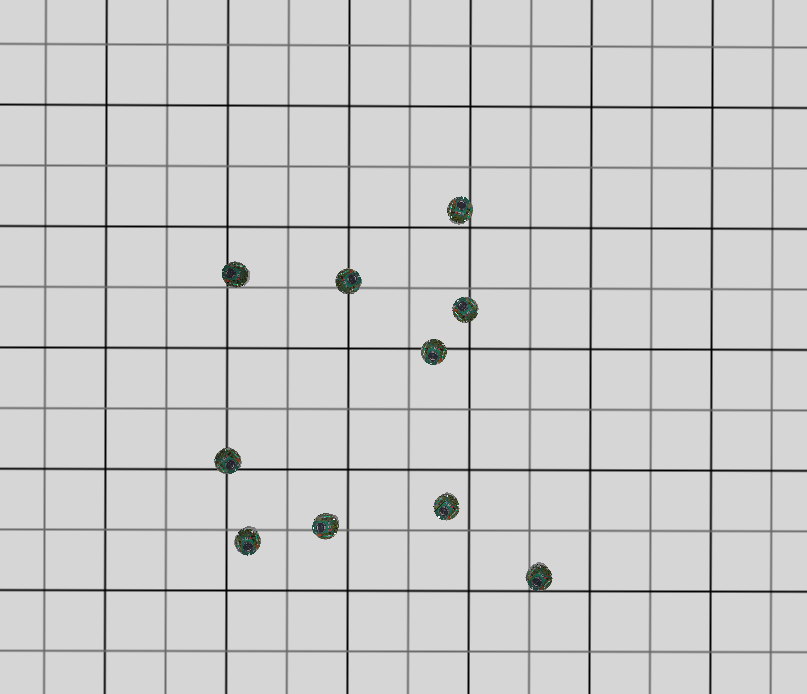
\includegraphics[width=8cm]{figures/swarm-10-screenshot.png}
      \caption{Realistic simulation in Webots}
    \end{center}
  \end{figure}

  \subsection{Macroscopic model}
  The macroscopic model of this wireless connected swarm is established from a set of differential equations (DE) described in \cite{Winfield08}. DEs precisely describe the rules governing state transitions at each timestep.\\

  The set of DEs can be separate into two hierarchical groups in a particle finite state machine (PFSM). In our case, the state machine has the following states:\\
  \begin{itemize}
    \item Forward (with subsumed state avoidance)
    \item Coherence (with subsumed state avoidance)
  \end{itemize}

  The sub-PFSM can be written simply from the conservation principle since the number of time steps to spend in avoidance is constant and known. The related terms are $N_F$, $N_{AF}$, $N_C$ and $N_{AC}$, for forward, avoidance-forward, coherence and avoidance-coherence states respectively.

  The PFSM can be expressed as the rate of change of the number of robots $N$ at state $X$ over timesteps $k$ for a given number of neighbors $i$:
  \[
    \frac{dN_{X_i}}{dt} \approx \frac{\Delta N_X}{\Delta_t} = N_{X_i}(k+1) - N_{X_i}(k)
  \]

  Then, the input and output for each DE are derived from the probability to change the state of a robot to X considering his current number of neighbors. The states $X$ are $N_{\bar F}$ and $N_{\bar C}$. There are six different state transition probabilities defined for the macroscopic model:

  \begin{table}[h]
    \begin{center}
      \begin{tabular}{r|l}
        \hline
        Notation   & Corresponding event \\
        \hline
        $P_a$      & go in avoidance \\
        $P_g$      & gain a connection in Forward \\
        $P_l$      & lost a connection in Forward \\
        $P_r$      & recover a connection in Coherence \\
        $P_f$      & fail to recover a connection in Coherence \\
        $P_{la}$   & lost a connection in Coherence \\
        \hline
      \end{tabular}
    \end{center}
  \end{table}

  Those probabilities were estimated from data collected from the submicroscopic simulations described in \ref{simulations} over 3 runs of $25 000$ timesteps. The probabilities are define as the total amount of robots that actually fulfilled the condition over the concerned population at $i$ connection. For instance, the probability to go in avoidance concerned the whole population at $i$ connection, when the probability to loose a connection in Forward only concerned the robots in Forward and Avoidance Forward states.

  The macroscopic model ran for $1000$ timesteps, estimating at each steps the number of robots for the next iteration in each state based on the set of DEs and the state transition probabilities, as rates of change coefficients:
  \[
    PY_i * N(X|PY)_i
  \]

  with $PY$ denoting any of the probabilities ($Y \in \{a, g, l, r, f, la\}$); and $N(X|PY)$ the number of robots in the affected state (knowing which one)

  For example, if we consider the state transition of robots which fail to recover a connection $Pf$, the related state knowing the consider probability $N(X|Pf)$ is the coherence state $N_{\bar C}$


\section{Results}
  On figure \ref{fig:main-results}, we compare the aggregated results of 10 runs of the submicroscopic model (left) with those of the macroscopic model (right). We are interested in the capacity of the macroscopic model to mimick the simulation runs.

  The results show the expected global tendency with a clearly visible mode centered on alpha. But some aspects aren't similar, the extremities dropped to zero too quickly, especially in the increasing side of the number of connections. As a consequence, the number of robots is higher than expected around the mode, in particular for the avoidance state. This could indicate a too low value for the rate of transition induced in the estimation of the transition state probabilities.\\

  To investigate the phenomena, the macroscopic model were tested using the results of \cite{Winfield08}, the model showed results similar to the article. This confirms the validity of the results as well as our implementation.

  Especially because this behavior still occurs for more calibration data and more simulation time steps, thus the generation of the probabilities is certainly the source of it.

  \begin{figure*}[p]
    \begin{center}
      \begin{tabular}{lr}
        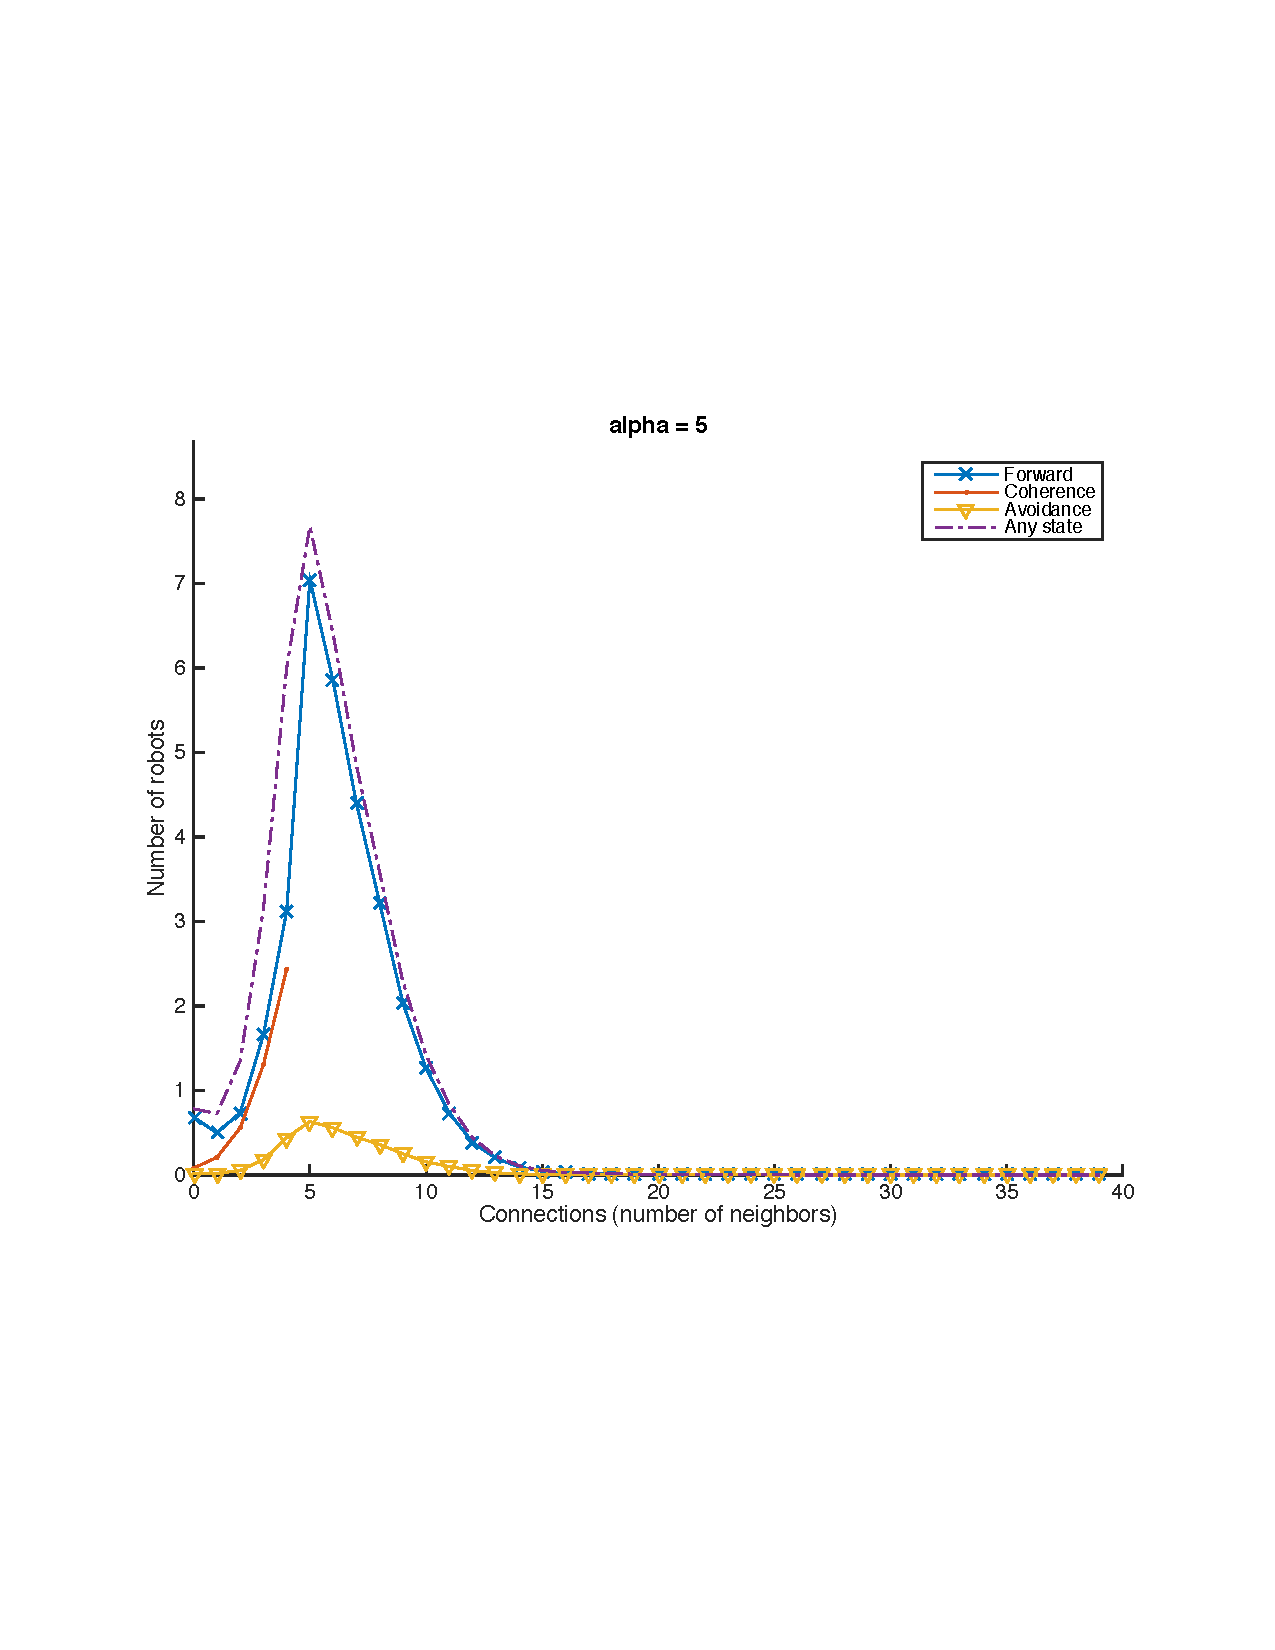
\includegraphics[width=8cm]{figures/simulation-40-alpha-5.pdf}   &
        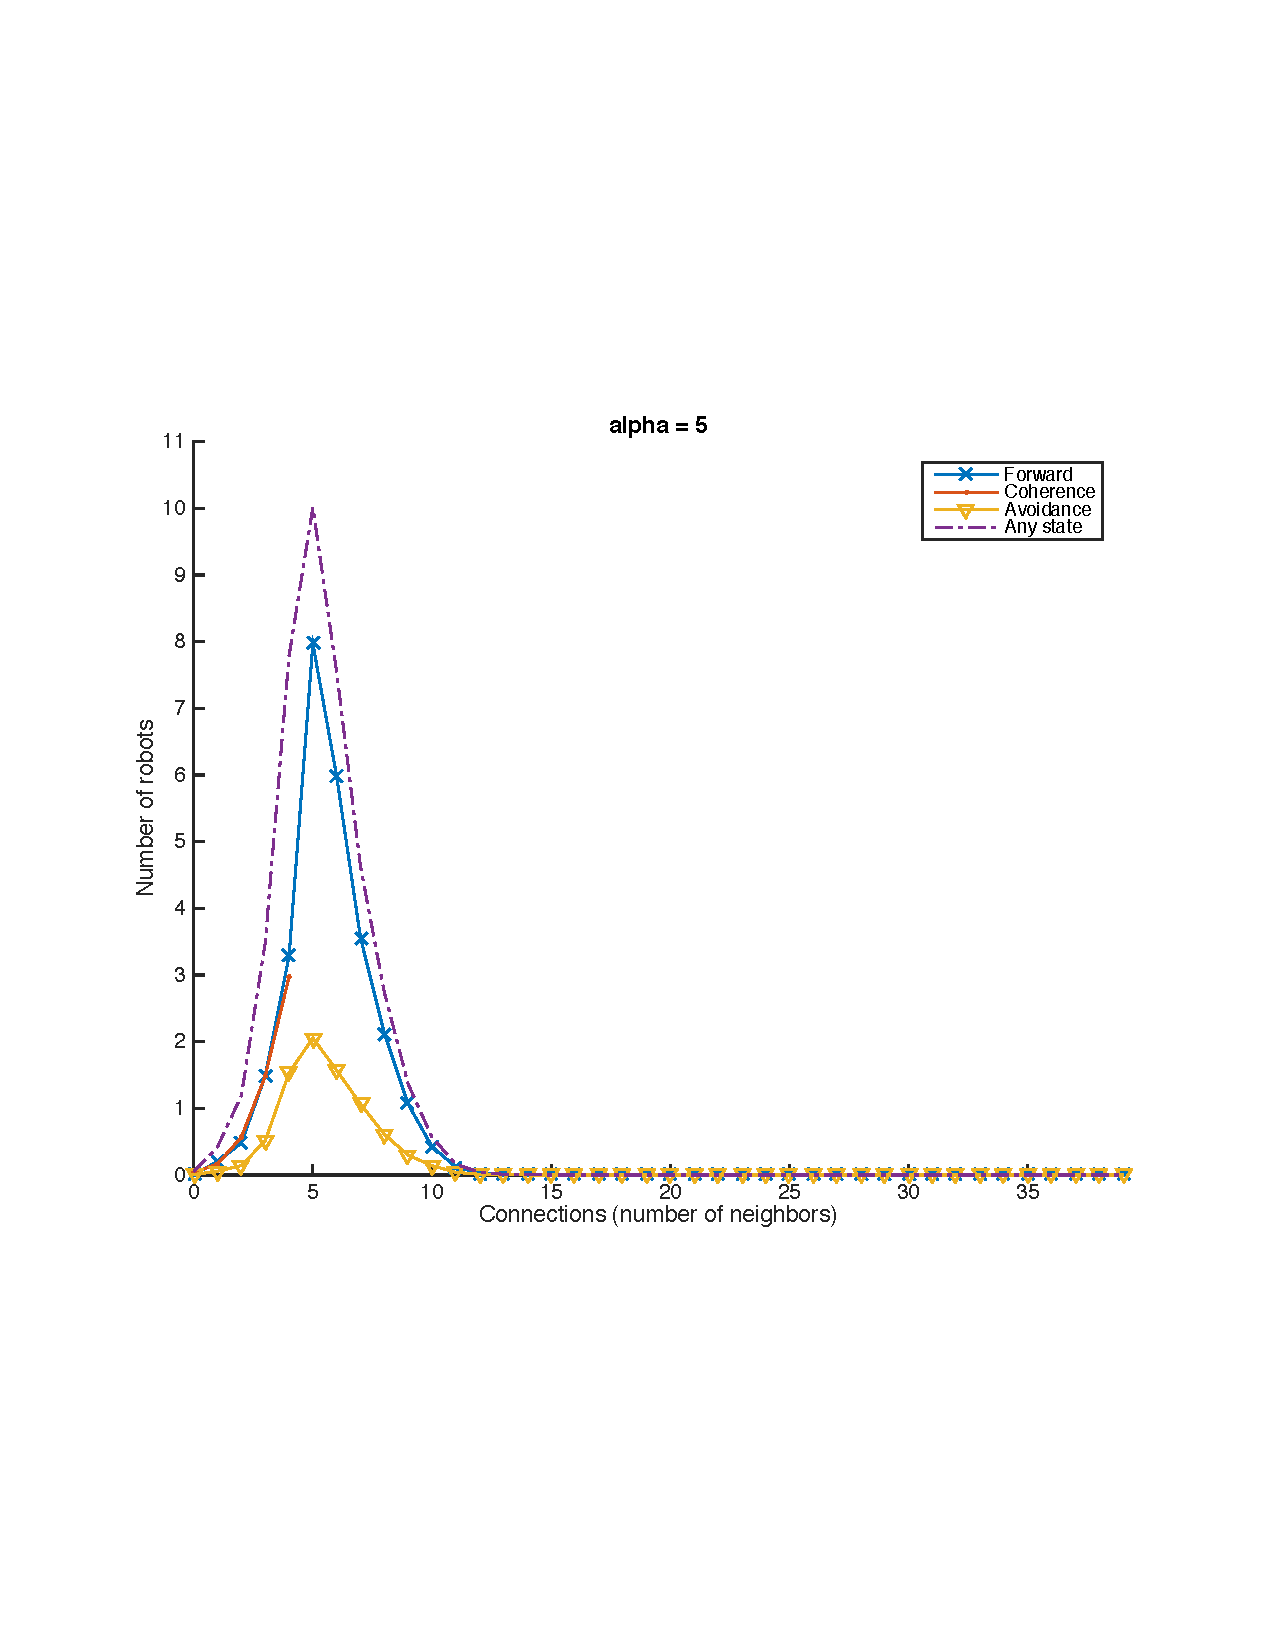
\includegraphics[width=8cm]{figures/macroscopic-40-alpha-5.pdf}  \\
        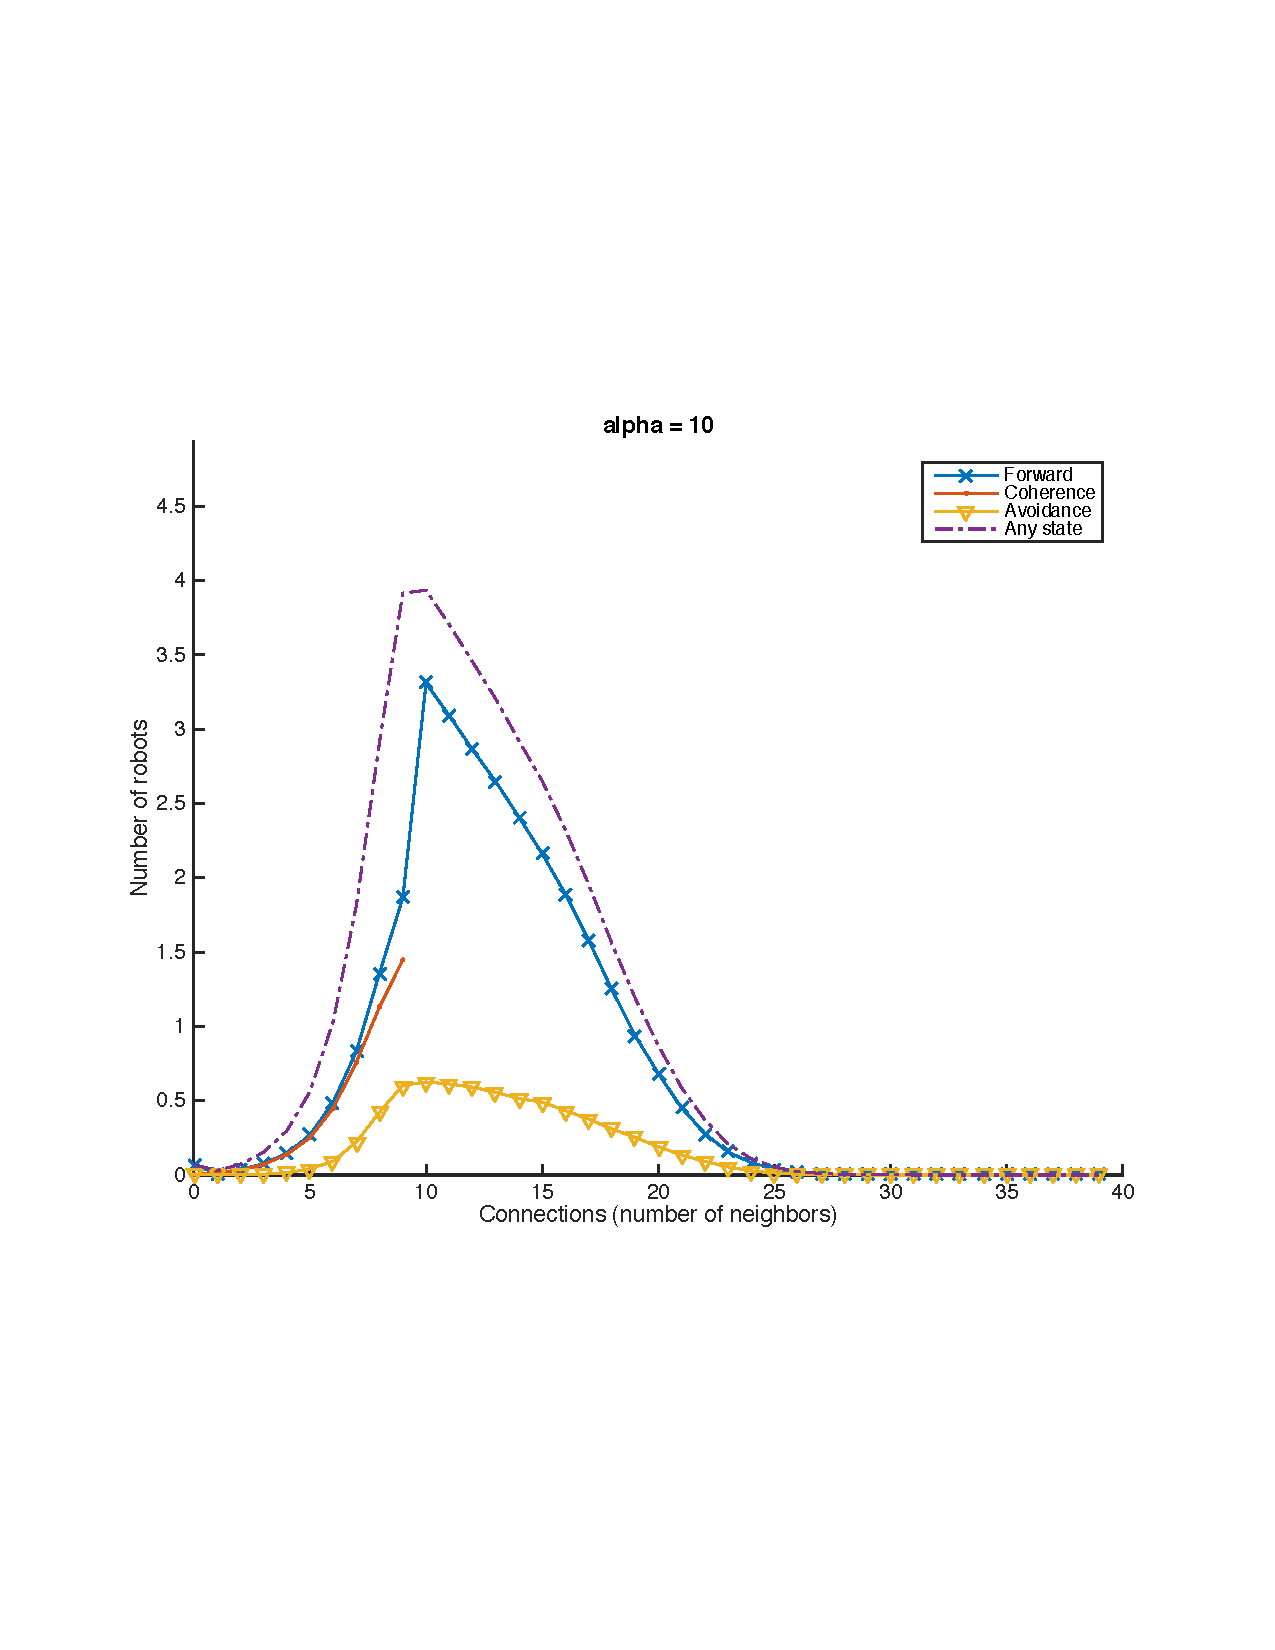
\includegraphics[width=8cm]{figures/simulation-40-alpha-10.pdf}  &
        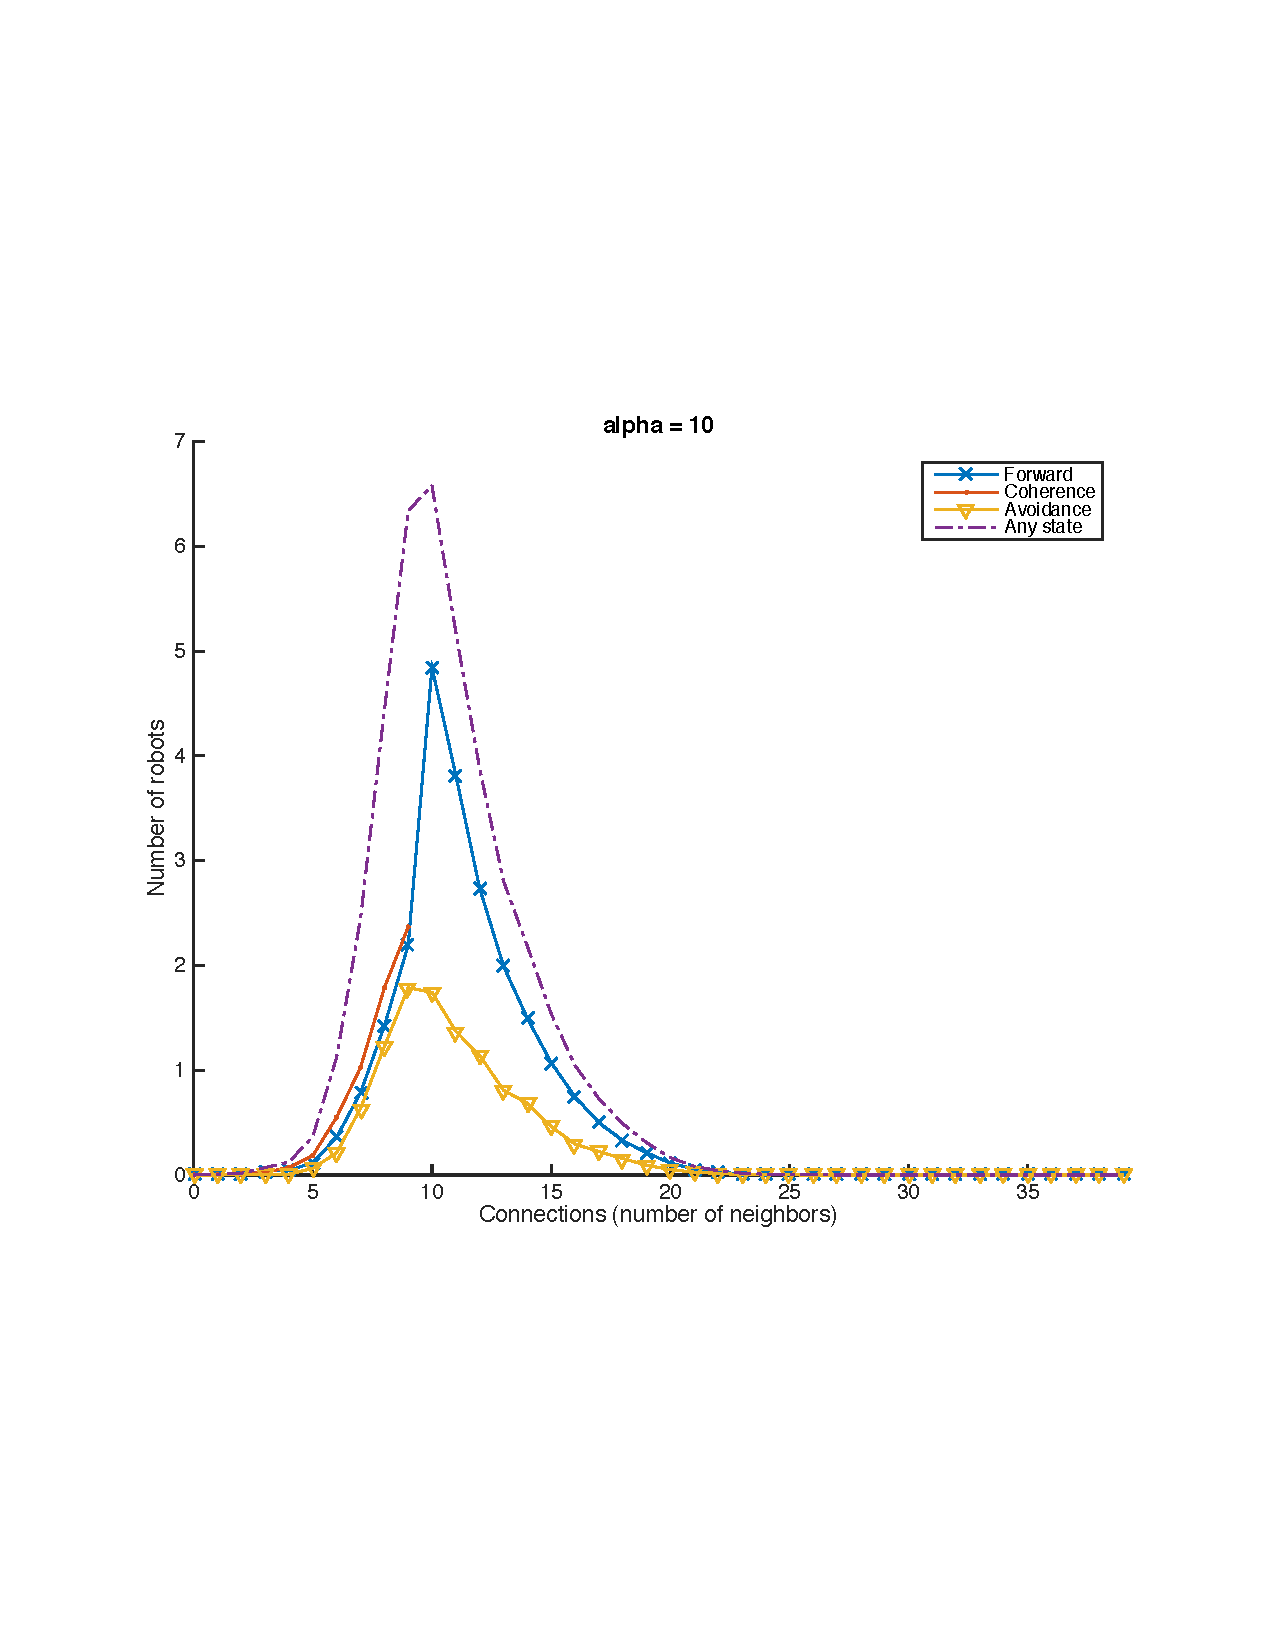
\includegraphics[width=8cm]{figures/macroscopic-40-alpha-10.pdf} \\
        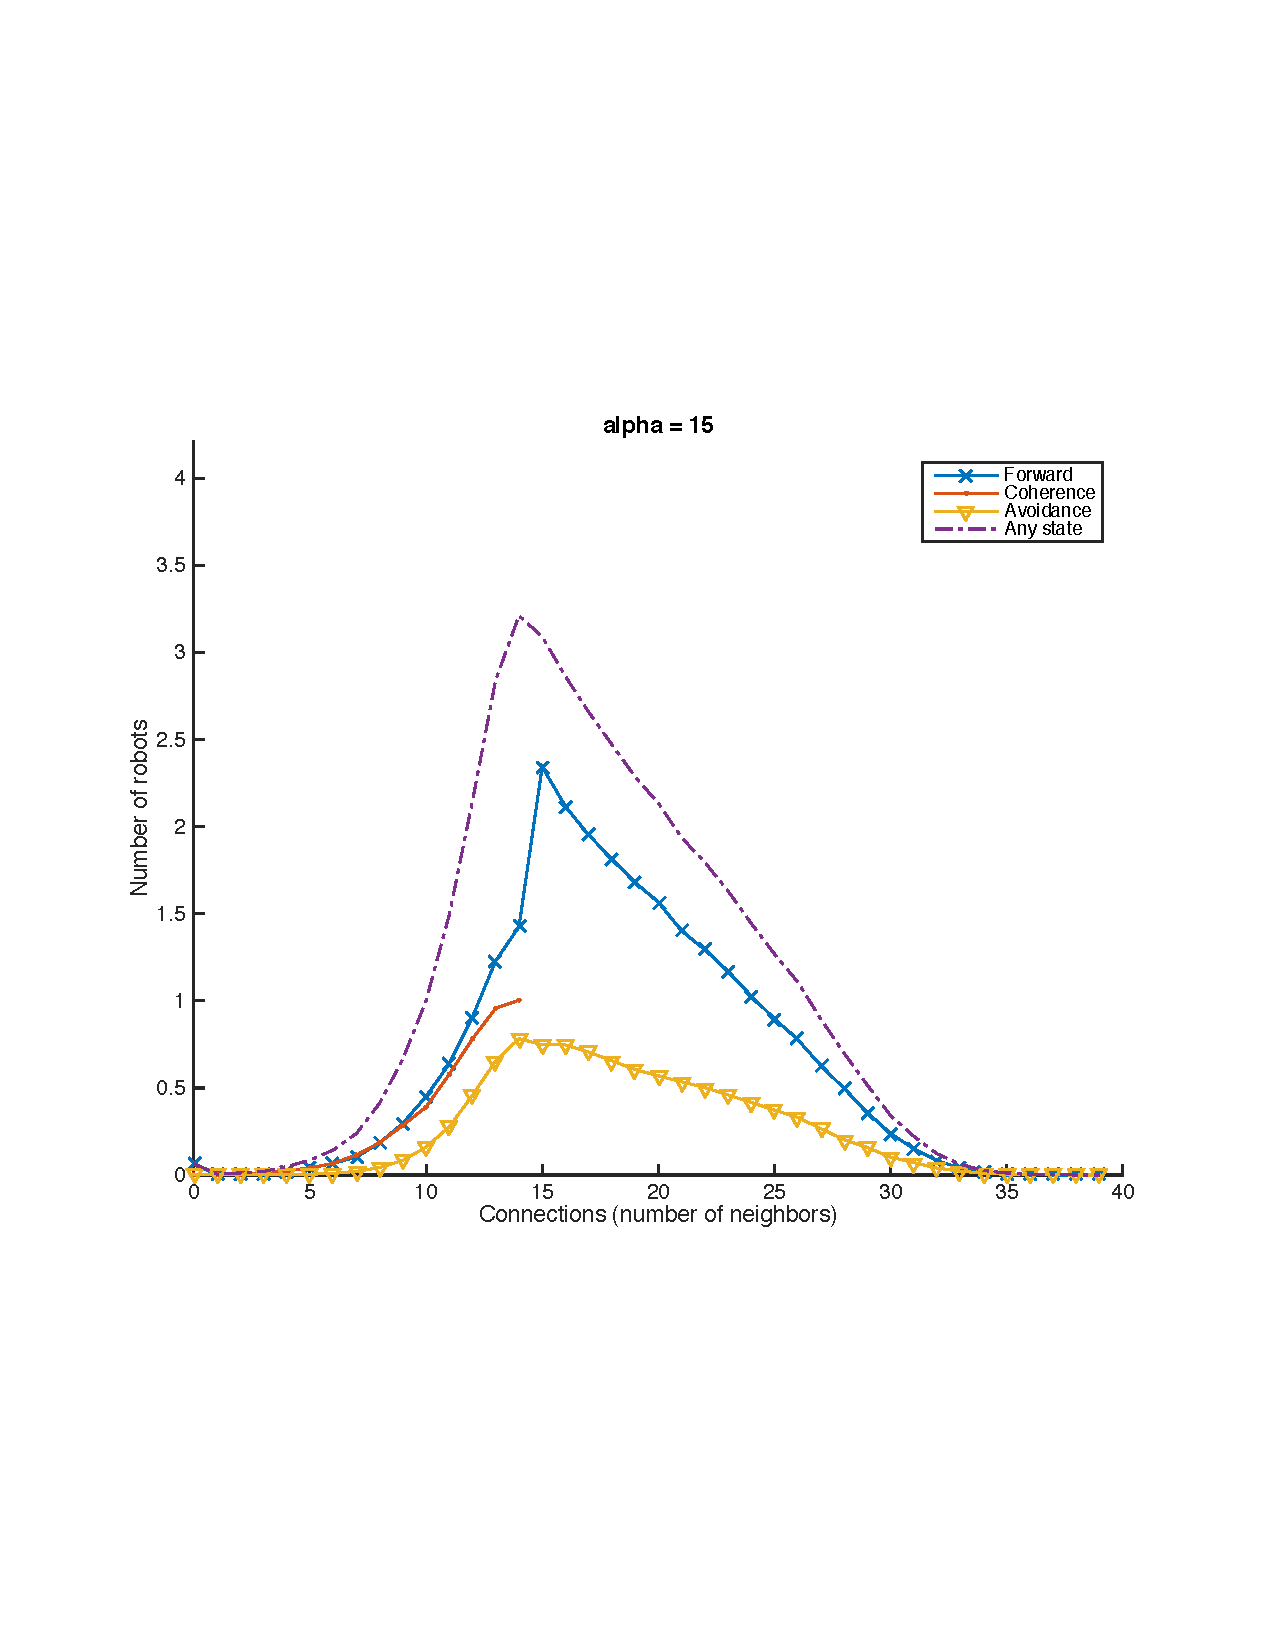
\includegraphics[width=8cm]{figures/simulation-40-alpha-15.pdf}  &
        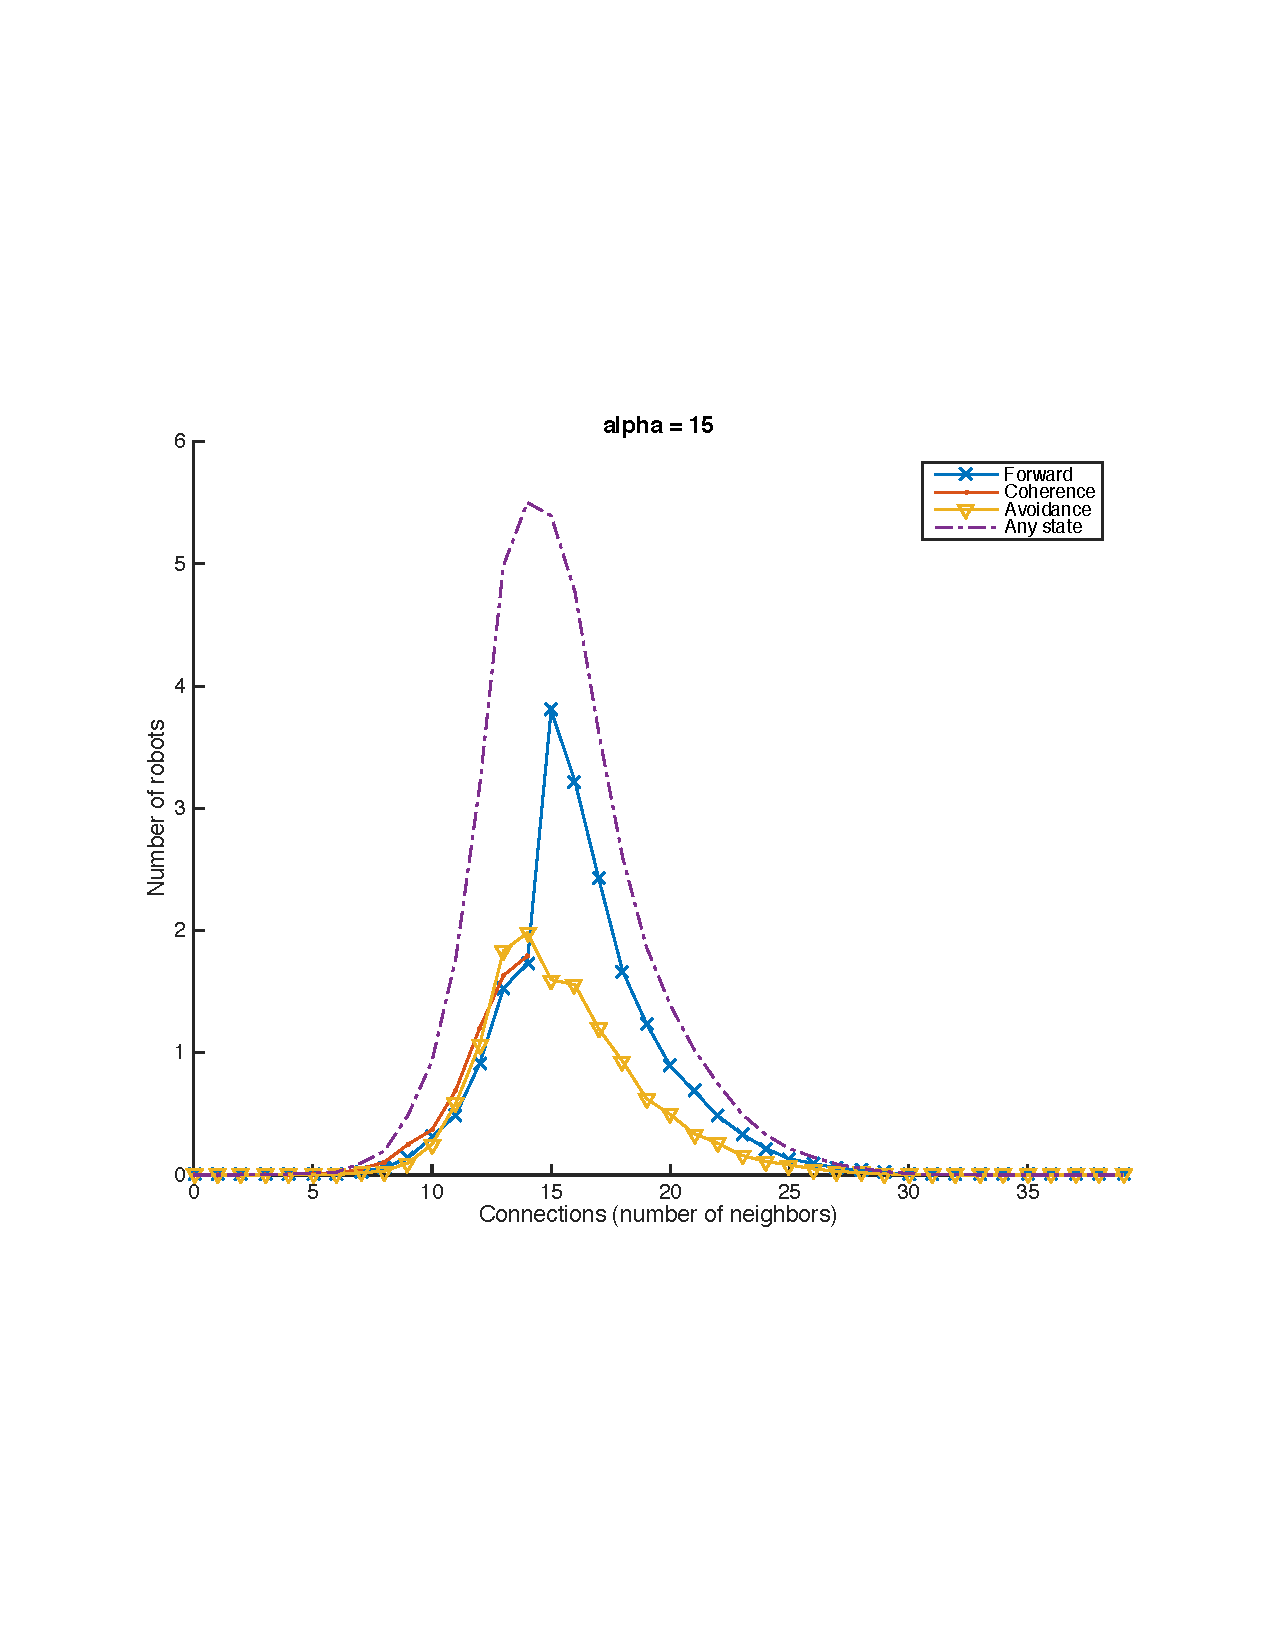
\includegraphics[width=8cm]{figures/macroscopic-40-alpha-15.pdf}
      \end{tabular}
      \caption{Results of realistic simulations (left) and macroscopic model (right) for $\alpha = 5$, $10$ and $15$ (from top to bottom). Values averaged over 10 runs are presented.}
      \label{fig:main-results}
    \end{center}
  \end{figure*}

%%%%%%%%%%%%%%%%%%%%%%%%%%%%%%%%%%%%%%%%%%%%%%%%%%%%%%%%%%%%%%%%%%%%%%%%%%%%%%%%

\section{Conclusion}

%%%%%%%%%%%%%%%%%%%%%%%%%%%%%%%%%%%%%%%%%%%%%%%%%%%%%%%%%%%%%%%%%%%%%%%%%%%%%%%%

%\addtolength{\textheight}{-12cm} % This command serves to balance the column lengths
                                  % on the last page of the document manually. It shortens
                                  % the textheight of the last page by a suitable amount.
                                  % This command does not take effect until the next page
                                  % so it should come on the page before the last. Make
                                  % sure that you do not shorten the textheight too much.

%%%%%%%%%%%%%%%%%%%%%%%%%%%%%%%%%%%%%%%%%%%%%%%%%%%%%%%%%%%%%%%%%%%%%%%%%%%%%%%%

\begin{thebibliography}{99}

  \bibitem{Nembrini02} Nembrini J, Winfield A and Melhuish C, \textit{Minimalist Coherent Swarming of Wireless Connected Autonomous Mobile Robots}, in Proc. Simulation of Artificial Behaviour '02, Edinburgh, August 2002.

  \bibitem{Winfield08} Winfield AFT, Liu W, Nembrini J and Martinoli A, \textit{Modelling a Wireless Connected Swarm of Mobile Robots}, Swarm Intelligence, 2 (2-4), 241-266, 2008.

\end{thebibliography}

\section*{Acknowledgments}
  We would like to thank our project supervisor Jose Nuno Pereira for his availability and helpful comments. We also thank Prof. Martinoli and his teaching assistants for holding lectures and labs which helped us gain a better understanding of multilevel modeling as well as implementation techniques.

\end{document}
